\def\level{BTS}  % Classe à droite
\def\course{CIEL 2}
\def\chaptername{Equations différentielles} % Titre au centre
\def\docpart{Equations différentielles~--~TP Géogébra 1} % Partie du cours
\def\docname{C215}        % Identifiant à gauche

\pagestyle{cours_FP}
\makeheaderBTS{} % Affiche le bandeau


\begin{exercice_cours}[\quad]{}

On considère l’équation différentielle (E) : $y' + 3y = 6e^{-x}$ où $y$ est une fonction de la variable réelle $x$, définie et dérivable sur l’ensemble $\R$ des nombres réels, et $y'$ est la fonction dérivée de $y$.

\begin{enumerate}
	\item Résoudre l'équation homogène (E$_0$) : $y'+3y=0$  \hfill\reponseLigne[7cm]{}
	\item A l’aide du logiciel Géogébra, déterminer les nombres réels $a$ et $b$ pour que la fonction $p$ définie sur $\R$ par : $p(x) = a + b~e^{- x}$ soit une solution particulière de l'équation différentielle (E), et donner l’expression de $p$. \hfill\reponseLigne[7cm]{}
	\item En déduire la forme générale des solutions de (E).  \hfill\reponseLigne[7cm]{}
	\item Déterminer, à l'aide de géogebra et d'un curseur bien choisi, la solution particulière $f$ de (E) telle que $f(0)=0$.  \hfill\reponseLigne[7cm]{}   
\end{enumerate}
\end{exercice_cours}
\begin{exercice_cours}[\quad]{}

	On considère l’équation différentielle (E) : $y' - y = 2e^{x}$ où $y$ est une fonction de la variable réelle $x$, définie et dérivable sur l’ensemble $\R$ des nombres réels, et $y'$ est la fonction dérivée de $y$.

\begin{enumerate}
	\item Résoure l'équation homogène (E$_0$) : $y'-y=0$  \hfill\reponseLigne[7cm]{}
	\item A l’aide du logiciel Géogébra, déterminer les nombres réels $a$ et $b$ pour que la fonction $p$ définie sur $\R$ par : $p(x) = ax~e^{x}$ soit une solution particulière de l'équation différentielle (E), et donner l’expression de $p$. \hfill\reponseLigne[7cm]{}
	\item En déduire la forme générale des solutions de (E).  \hfill\reponseLigne[7cm]{}
	\item Déterminer, à l'aide de géogebra et d'un curseur bien choisi, la solution particulière $f$ de (E) telle que $f(0)=-1$.      \hfill\reponseLigne[7cm]{}
\end{enumerate}
\end{exercice_cours}
\begin{exercice_cours}[\quad]{}

	On considère l’équation différentielle (E) : $y' + 4y = 8-3e^{-4x}$ où $y$ est une fonction de la variable réelle $x$, définie et dérivable sur l’ensemble $\R$ des nombres réels, et $y'$ est la fonction dérivée de $y$.

\begin{enumerate}
	\item Résoure l'équation homogène (E$_0$) : $y'+4y=0$     \hfill\reponseLigne[7cm]{}
	\item A l’aide du logiciel Géogébra, déterminer les nombres réels $a$ et $b$ pour que la fonction $p$ définie sur $\R$ par : $p(x) = a + b~x~e^{-4x}$ soit une solution particulière de l'équation différentielle (E), et donner l’expression de $p$.  \hfill\reponseLigne[7cm]{}  
	\item En déduire la forme générale des solutions de (E).  \hfill\reponseLigne[7cm]{}
	\item Déterminer, à l'aide de géogebra et d'un curseur bien choisi, la solution particulière $f$ de (E) telle que $f(0)=2$.  \hfill\reponseLigne[7cm]{}    
\end{enumerate}
\end{exercice_cours}
\begin{exercice_cours}[\quad]{}

	On considère l’équation différentielle (E) : $2y' + y = e^{-0,5x}$ où $y$ est une fonction de la variable réelle $x$, définie et dérivable sur l’ensemble $\R$ des nombres réels, et $y'$ est la fonction dérivée de $y$.

\begin{enumerate}
	\item Donner et résoudre l'équation homogène (E$_0$)  	    \hfill\reponseLigne[7cm]{}
	\item Démontrer, par un calcul, que la fonction $p$ définie sur $\R$ par : $p(x) = 0,5~x~e^{-0,5x}$ est une solution particulière de l'équation différentielle (E)  \hfill\reponseLigne[7cm]{}
	\item En déduire la forme générale des solutions de (E).    \hfill\reponseLigne[7cm]{}
	\item Déterminer, à l'aide de géogebra et d'un curseur bien choisi, la solution particulière $f$ de (E) telle que $f(0)=1$.   \hfill\reponseLigne[7cm]{}
\end{enumerate}
\end{exercice_cours}
\begin{exercice_cours}[\quad]{}

	On considère l’équation différentielle (E) : $y' + y = 1-e^{-x}$ où $y$ est une fonction de la variable réelle $x$, définie et dérivable sur l’ensemble $\R$ des nombres réels, et $y'$ est la fonction dérivée de $y$.

\begin{enumerate}
	\item Donner et résoudre l'équation homogène (E$_0$)  	\hfill\reponseLigne[7cm]{}    
	\item A l’aide du logiciel Géogébra, déterminer les nombres réels $a$ et $b$ pour que la fonction $p$ définie sur $\R$ par : $p(x) = a + b~x~e^{-x}$ soit une solution particulière de l'équation différentielle (E), et donner l’expression de $p$.    \hfill\reponseLigne[7cm]{} 	
	\item En déduire la forme générale des solutions de (E).  \hfill\reponseLigne[7cm]{}
	\item Déterminer, à l'aide de géogebra et d'un curseur bien choisi, la solution particulière $f$ de (E) telle que $f'(0)=0$.  \hfill\reponseLigne[7cm]{}
\end{enumerate}
\end{exercice_cours}
\begin{exercice_cours}[\quad]{}

	Un condensateur de capacité C $= 15\times10^{-5}$ Farads, initialement chargé à une tension de 10 Volts, se décharge à partir de l'instant $t_0=0$ à travers un circuit de résistance R$ = 2\times10^4$ Ohms. 

    

On sait que la tension $u$ est une fonction de la variable réelle $t$, exprimée en seconde, solution de l'équation différentielle suivante :

\[(E) : \qquad R~C~\dfrac{\text{d}u}{\text{d}t}(t)+u(t)=0\]



\begin{enumerate}
	\item Justifier que (E) peut s'écrire : $3u'+u=0$  \hfill\reponseLigne[7cm]{}  
	\item Résoudre l'équation homogène (E) \hfill\reponseLigne[7cm]{}
	\item Justifier que $u(0)=10$    \hfill\reponseLigne[7cm]{}
	\item Déterminer, par un calcul, la solution $u$ de (E) telle que $u(0)=10$.    
		\begin{blocvisiblex}[height=2]
{\quad}

\end{blocvisiblex}
	\item À l'aide de Géogebra, déterminer à partir de quel instant, que l'on notera $t_1$, $u(t)\leq \dfrac{10}{100}u_0$ ?
	\hfill\reponseLigne[7cm]{}
	    
	
	    
	\item On rappelle que la valeur moyenne d'une fonction $f$ entre $a$ et $b$, vaut ${\dfrac{1}{b-a}\int_a^bf(x)\text{d}x}$
	\begin{enumerate}
		\item Rappeler la formule permettant de calculer $ {\int_a^bf(x)\text{d}x}$ à l'aide d'une primitive F de $f$.     
		
		\hfill\reponseLigne[7cm]{}
		\item Déterminer une primitive U de $u$.   \hfill\reponseLigne[7cm]{} 
		\item À l'aide de Geogebra, donner une valeur approchée, au dixième de Volt près, de la valeur moyenne de la tension $u$ entre les instants $t_0$ et $t_1$.    
		
		\hfill\reponseLigne[7cm]{}
	\end{enumerate}
\end{enumerate}
\end{exercice_cours}
\begin{exercice_cours}[\quad]{}

	On applique une tension $t\mapsto 5+\e^{-t}$ aux bornes d'un circuit. Le courant vérifie l'équation différentielle : $y'+5y=5+\e^{-t}$

\begin{enumerate}
	\item Donner et résoudre l'équation homogène (E$_0$)    \hfill\reponseLigne[7cm]{}
	\item A l’aide du logiciel Géogébra, déterminer les nombres réels $a$ et $b$ pour que la fonction $p$ définie sur $\R$ par : $p(x) = a + b~\e^{-t}$ soit une solution particulière de l'équation différentielle (E), et donner l’expression de $p$. \hfill\reponseLigne[7cm]{}
	\item En déduire la forme générale des solutions de (E).  \hfill\reponseLigne[7cm]{}  
\end{enumerate}
\end{exercice_cours}


\begin{exercice_cours}[\quad]{}

	Dans ce problème, on se propose d’étudier l’évolution de la concentration dans le sang d’un médicament ingéré par une personne pour la première fois.

	\medskip

{\bf Partie A}\par     

Soit $t$ le temps (exprimé en heures) écoulé depuis l’ingestion de ce produit. Cette concentration, en gramme par litre de sang, est une fonction $f$ de la variable $t$ définie sur l’intervalle $[0~;~+\infty[$ qui est solution de l’équation différentielle :

\[(E) : \quad y'(t)+y(t)= a\e^{-t} \]

Avec $a$ est une constante positive dépendant de la personne et de la quantité de médicament absorbée, et avec la condition initiale : $f (0) = 0$.

On suppose ici que $a = 5$, l’équation (E) s’écrit alors : $y'(t)+y(t)= 5\e^{-t}$

\begin{enumerate}
	\item Donner, puis résoudre l'équation homogène (E$_0$): 
	
	\hfill\reponseLigne[0.95\linewidth]{}   	    
	\item A l’aide du logiciel Géogébra, déterminer le nombre réel $m$ pour que la fonction $p$ définie sur $[0~;~+\infty[$ par : $p(t) = m~t~\e^{-t}$ soit une solution particulière de l'équation différentielle (E), et donner l’expression de $p$. 	\hfill\reponseLigne[7cm]{}
	\item En déduire l'ensemble des solutions de (E):     \hfill\reponseLigne[7cm]{}
	\item Déterminer, par un calcul, la solution $f$ de (E) répondant aux contraintes de l'énoncé :     
\begin{blocvisiblex}[height=2]
{\quad}
\end{blocvisiblex}
\end{enumerate}

\pagebreak

{\bf Partie B}\par     

On considère la fonction $f$ définie sur $[0~;~+\infty[$ par : $f(t)=5~t~\e^{-t}$

\begin{enumerate}
	\setcounter{enumi}{4}
	\item À l'aide de l'outil calcul formel de Géogebra, étudier les varations de $f$ sur $[0~;~+\infty[$ :
	
	\begin{enumerate}
		\item Déterminer $f'(t)$.\hfill\reponseLigne[7cm]{}   
		
		\item Résoudre sur $\left[0~;~+\infty\right[$ : $f'(t)=0$ \hfill\reponseLigne[7cm]{}   
		
		\item \hspace*{4.2cm}$f'(t)\geq 0$ \hfill \reponseLigne[7cm]{}    
		
		\item Compléter alors le tableau de variation complet de la fonction $f$ sur $\left[0~;~+\infty\right[$ :
		
		{\it \small On fera figurer les valeurs au bout des flèches}
		
		\begin{center}
		\begin{tikzpicture}
	   \tkzTabInit[lgt=3]{$t$ / 1 , signe de $f'(t)$ / 1, variations de $f$ / 2}{$ $, $ $, $ $, $ $}
		\end{tikzpicture}	
		\end{center}
		\end{enumerate}	
	
	\item On a ${\displaystyle\lim_{t\rightarrow+\infty}f(t)=0}$. Comment interpréter médicalement ce résultat ?    

	\begin{blocvisiblex}[height=2]
{\quad}
\end{blocvisiblex}
	    
	\item Pour une concentration supérieur à 1 gramme par litre de sang, il y a risque de somnolence.
	
	Déterminer, à l’aide de la courbe de f, combien de temps après la prise du médicament le risque de somnolence n’est plus. Donner le résultat en heures et minutes.    

	    \begin{blocvisiblex}[height=2]
{\quad}
\end{blocvisiblex}
\end{enumerate}

{\bf Partie C}

\begin{enumerate}
	\setcounter{enumi}{7}
	\item Soit $F$ la fonction définie sur $\left[0~;~+\infty\right[$ par : $F(t)=(-5~t-5)\e^{-t}$
	\begin{enumerate}
		\item Vérifier, par un calcul, que $F$ est une primitive de $f$.     

		\begin{blocvisiblex}[height=3]
{\quad}
\end{blocvisiblex}
	    
		
		\item La concentration moyenne du médicament (en gramme par litre de sang) durant la première heure est donnée par : $ {T_m = \int_0^1f(t)\text{d}t}$
		
		Rappeler la formule permettant de calculer $T_m$ à l'aide de $F$, puis donner une valeur approchée à $0,01$ près.    

\begin{blocvisiblex}[height=2]
{\quad}
\end{blocvisiblex}
	\end{enumerate}
\end{enumerate}
\end{exercice_cours}

\begin{exercice_cours}[\quad]{}

	On considère l’équation différentielle (E) : $y' + 2y = 3x+2$ où $y$ désigne une fonction de la variable réelle $x$ définie et dérivable sur $\R$, $y'$ sa fonction dérivée.

\begin{enumerate}
	\item Donner, puis résoudre l'équation homogène (E$_0$):\hfill\reponseLigne[7cm]{}  
	\item A l’aide du logiciel Géogébra, déterminer les nombres réels $a$ et $b$ pour que la fonction $p$ définie sur $\R$ par : $p(x) = ax+b$ soit une solution particulière de (E), et donner l’expression de $p$. \par\hfill\reponseLigne[7cm]{}
	\item En déduire l'ensemble des solutions de (E):   \hfill\reponseLigne[7cm]{}   
	\item Déterminer, par un calcul, la solution $f$ de (E) telle que $f(0)=2$ :   
\begin{blocvisiblex}[height=2]
{\quad}
\end{blocvisiblex}
\end{enumerate}
\end{exercice_cours}
\begin{exercice_cours}[\quad]{}

	On considère l’équation différentielle (E) : $y' - y = 2(x + 1)\e^x$ où $y$ désigne une fonction de la variable réelle $x$ définie et dérivable sur $\R$, $y'$ sa fonction dérivée.

\begin{enumerate}
	\item Donner, puis résoudre l'équation homogène (E$_0$):  \hfill\reponseLigne[7cm]{}
	\item A l’aide du logiciel Géogébra, déterminer les nombres réels $a$ et $b$ pour que la fonction $p$ définie par : $p(x) = (a~x^2+b~x)\e^x$ soit une solution particulière de (E), et donner l’expression de $p$. \par \hfill\reponseLigne[7cm]{}
	\item En déduire l'ensemble des solutions de (E): \hfill\reponseLigne[7cm]{}   	    
	\item Déterminer, par un calcul, la solution $f$ de (E) telle que $f'(0)=3$ : 	
\begin{blocvisiblex}[height=2]
{\quad}
\end{blocvisiblex}
\end{enumerate}
\end{exercice_cours}
\begin{exercice_cours}[\quad]{}

	On considère l’équation différentielle (E) : $y' - y = 2(x + 1)\e^x$ où $y$ désigne une fonction de la variable réelle $x$ définie et dérivable sur $\R$, $y'$ sa fonction dérivée.

\begin{enumerate}
	\item Donner, puis résoudre l'équation homogène (E$_0$):  \hfill\reponseLigne[7cm]{}
	\item Vérifier que la fonction $p(x)=(x^2+2x)\e^{x}$ est une solution particulière de (E). 
	\begin{blocvisiblex}[height=2]
{\quad}
\end{blocvisiblex}
\item En déduire l'ensemble des solutions de (E):    \hfill\reponseLigne[7cm]{}
	\item Déterminer, à l'aide de géogebra et d'un curseur bien choisi, la solution particulière $f$ de (E) telle que $f'(0)=3$.   \hfill\reponseLigne[7cm]{}
\end{enumerate}
\end{exercice_cours}
\begin{exercice_cours}[\quad]{}

	Le but du problème est l’étude de la demande et de l’offre pour un nouveau produit
de grande consommation.

\begin{itemize}
	\item $x$ désigne le prix unitaire en euros du produit ;
	\item $f$ désigne la demande (la quantité de produit demandée par les consommateurs),
en milliers d’unités ;
	\item $h$ désigne l’offre (la quantité de produit offerte sur le marché par les producteurs),
en milliers d’unités.
\end{itemize}


	On considère l’équation différentielle (E) : $y' + 0,4 y = 0,4x-1$ où $y$ désigne une fonction de la variable réelle $x$ définie et dérivable sur $\R$, $y'$ sa fonction dérivée.

\begin{enumerate}
	\item Donner, puis résoudre l'équation homogène (E$_0$):   \hfill\reponseLigne[7cm]{}
	\item A l’aide de Géogébra, déterminer les réels $a$ et $b$ pour que la fonction $p$ définie par : $p(x) = a~x+b$ soit une solution particulière de l'équation différentielle (E), et donner l’expression de $p$. \par  \hfill\reponseLigne[7cm]{}
	\item En déduire l'ensemble des solutions de (E):    \hfill\reponseLigne[7cm]{}
	\item \begin{enumerate}
		\item Déterminer, par un calcul, la solution $f$ de (E) telle que $f(0)=10$:   
		\begin{blocvisiblex}[height=2]
{\quad}
\end{blocvisiblex}
\item Interpréter, dans le contexte de l'énoncé, la condtion initiale $f(0)=10$ :  
	\begin{blocvisiblex}[height=2]
{\quad}
\end{blocvisiblex}
\end{enumerate}
	\item L'offre est représentée par la fonction $h(x) = \ln(3x + 0, 9)$. Le prix de vente est fixé comme la valeur de $x$ pour laquelle l'offre est égale à la demande.
	
	À l'aide de Géogebra, déterminer le prix de vente du produit :  \hfill\reponseLigne[5cm]{}
	

\end{enumerate}
\end{exercice_cours}